109. \begin{figure}[ht!]
\center{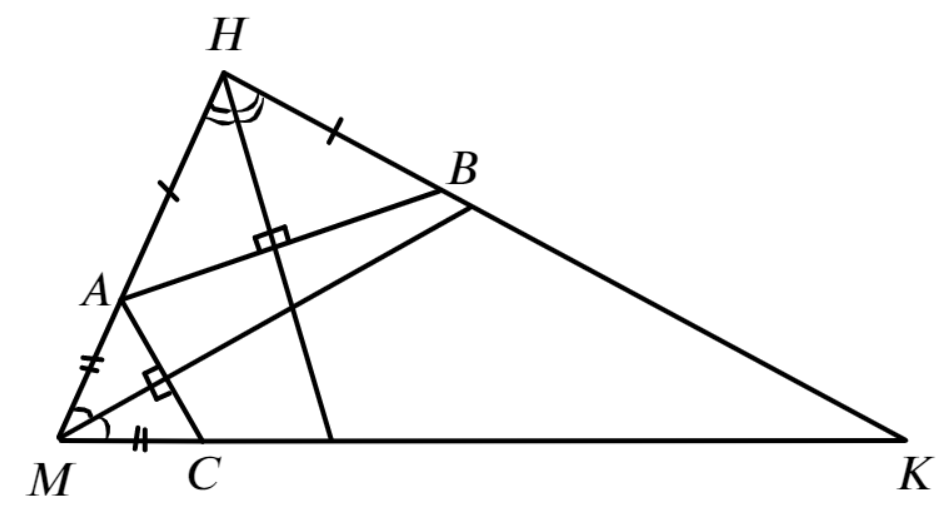
\includegraphics[scale=0.35]{g109.png}}
\end{figure}\\
В треугольниках $AHB$ и $MAC$ высота совпадает с биссектрисой, значит они равнобедренные. Введём обозначения $AH=HB=x,\ MA=MC=y,\ KB=z,\ KC=2z.$ Тогда получаем систему уравнений $\begin{cases} x+y=9,\\ x+z=12,\\ y+2z=18.\end{cases}$ Домножим второе уравнение на 2, сложим с первым и вычтем третье, получим $2x+2z+x+y-y-2z=24+9-18,\ 3x=15,\ x=5.$ Тогда $y=9-5=4$ и отношение равно $5:4.$\\
